\documentclass{article}
\usepackage[utf8]{inputenc}
\usepackage{graphicx}
\usepackage{pgfgantt}
\usepackage{lscape}
\usepackage{rotating}
\renewcommand{\refname}{Kaynakça}
\usepackage{pdflscape}
\usepackage{hyperref}
\usepackage{caption}

\DeclareCaptionLabelFormat{custom}{\textbf{Figür #2}}
\captionsetup[figure]{labelformat=custom,labelsep=period}

\begin{document}

\begin{titlepage}
    \centering
    %\vspace*{0.5cm}
    
\includegraphics[width=0.3\textwidth]{ksbu.png} 
    \vskip 1em
    \vspace{1cm}
    {\scshape\Large ML-Agents Rapor \par}
    \vspace{1cm}
    {Yazar: Mert Koca \par}
    {\today\par}
    %\vfill
    \begin{center}
        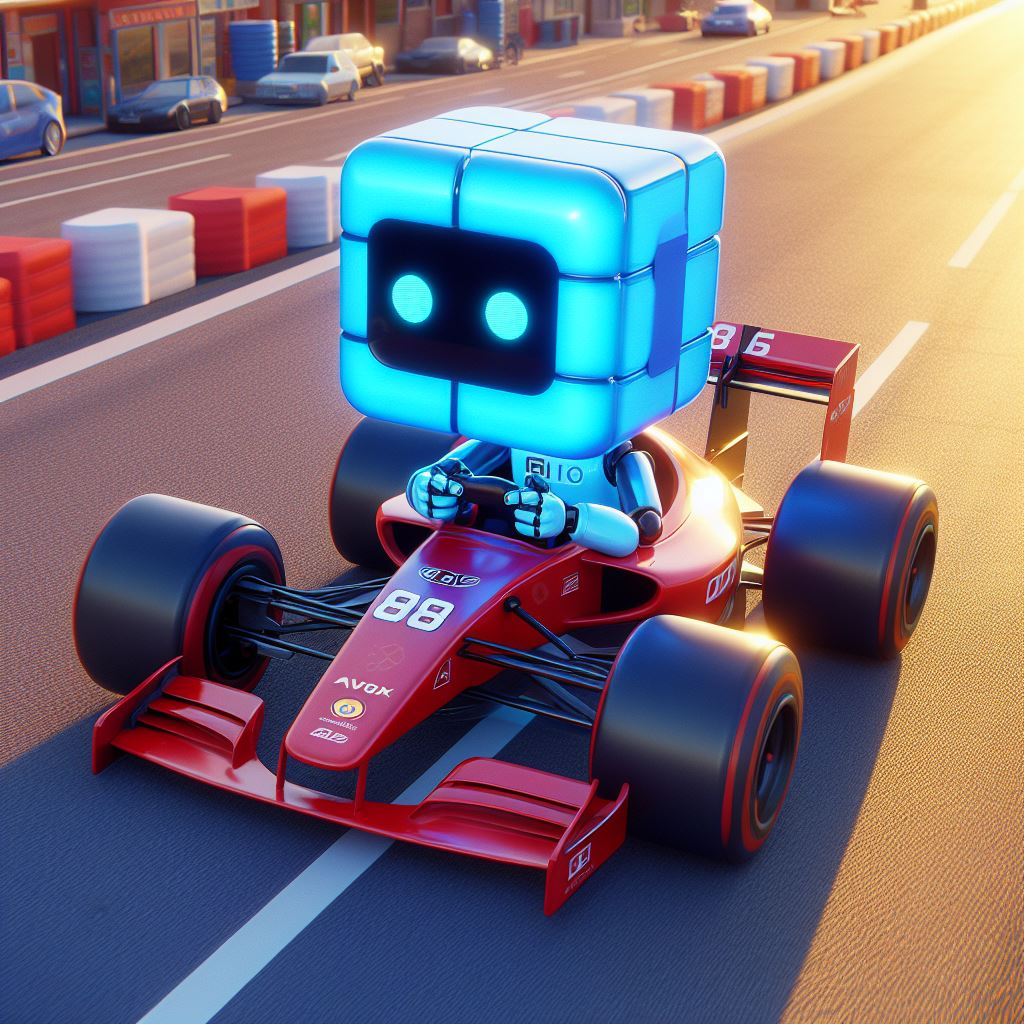
\includegraphics[width=0.5\textwidth]{gorsel.jpeg} 
    \end{center}
    \vspace{0.5cm}
    {Özet \par}
    \vspace{0.1cm}
    {Bu proje, Unity'nin ML-Agents kütüphanesi kullanılarak Python ve PyTorch ile geliştirilen bir yapay zeka projesidir. Bu proje, Unity ortamında eğitilmiş bir yapay zeka modeli oluşturarak araba sürmeyi öğretmeyi amaçlamaktadır.\par}
    \vspace{1cm}
\end{titlepage}

\newpage

\section{Giriş}
\rule{\textwidth}{0.5pt}
\par Bu rapor, Unity'nin ML-Agents kütüphanesi kullanılarak Python ve PyTorch ile geliştirilen bir yapay zeka projesine odaklanmaktadır. Proje, yapay zeka modellerinin eğitimini sağlamak amacıyla Unity ortamında bir simülasyon üzerinde çalışmaktadır. Hedef, araç sürmeyi öğrenen ve geliştiren bir yapay zeka modeli oluşturmaktır. Bu rapor, projenin amaçlarını, gereksinimlerini, kullanılan literatürü, algoritmaları, kurulum adımlarını, bileşenleri, bölüm tasarımını, kontrolleri ve sonuçları detaylı bir şekilde sunmaktadır.

\section{Gereksinimler}
\rule{\textwidth}{0.5pt}
\begin{enumerate}
    \item Python 3.9.13
    \item Unity
    \item PyTorch
    \item Visual Studio  
    \item ML-Agents Kütüphanesi\\[5pt]
\end{enumerate}

\section{Literatür}
\rule{\textwidth}{0.5pt}
\par \textbf{Python 3.9.13:} Genel amaçlı, yüksek seviyeli, etkileşimli bir programlama dilidir. Basit ve okunabilir sözdizimine sahiptir. Python, modüler yapısı ve geniş standart kütüphanesiyle birçok farklı alanda kullanılabilir.\\[5pt]

\textbf{PyTorch:} Python tabanlı ve açık kaynaklı makine öğrenmesi kütüphanesidir.\\[5pt]

\textbf{Unity:} Oyun ve grafik uygulamaları geliştirmek için kullanılan bir oyun motorudur.\\[5pt]

\textbf{ML-Agents Kütüphanesi:} Oyun ve simülasyonlarda ajanların eğitimi için ortamlar sağlayan açık kaynaklı bir projedir. Python API'ı kullanılarak teşvik öğrenmesi yöntemiyle ajanlar eğitilebilir. PyTorch tabanlı uygulamalar sunar. Ajanlar, NPC davranışlarını kontrol etmek ve oyun yapılarının otomatik test edilmesi gibi çeşitli amaçlar için kullanılabilir.


\section{Teşvik Öğrenme Algoritması}
\rule{\textwidth}{0.5pt}
\par Teşvik öğrenme algoritmasında, ajan çevresiyle etkileşime girer, belirli eylemler gerçekleştirir ve bu eylemlerin sonuçlarına göre ödüller veya ceza alır. Resimde gösterilen şema, ajanın çevresiyle olan etkileşimini ve bu süreçteki temel unsurları açıkça göstermektedir. Ajan, deneyimlediği ödül ve cezaları kullanarak en iyi eylem stratejilerini geliştirmeye çalışır.
\newline
\par Ibrahim Sobh Ibrahim'in yürüttüğü araştırma\cite{kiran2021deep}, Reinforcement Learning (RL) algoritmalarını kullanarak ajanların dinamik ortamlarda hızlı bir şekilde öğrenmesini ve adapte olmasını vurgulamaktadır. Derin RL'yi kullanarak, çalışma, özellikle müzakere gerektiren ve dinamik etkileşimler gerektiren senaryolarda otonom ajanların karar verme yeteneklerini artırmayı amaçlamaktadır.r verme yeteneklerini artırmayı amaçlamaktadır.\\[5pt]

\begin{figure}[h]
    \begin{center}
        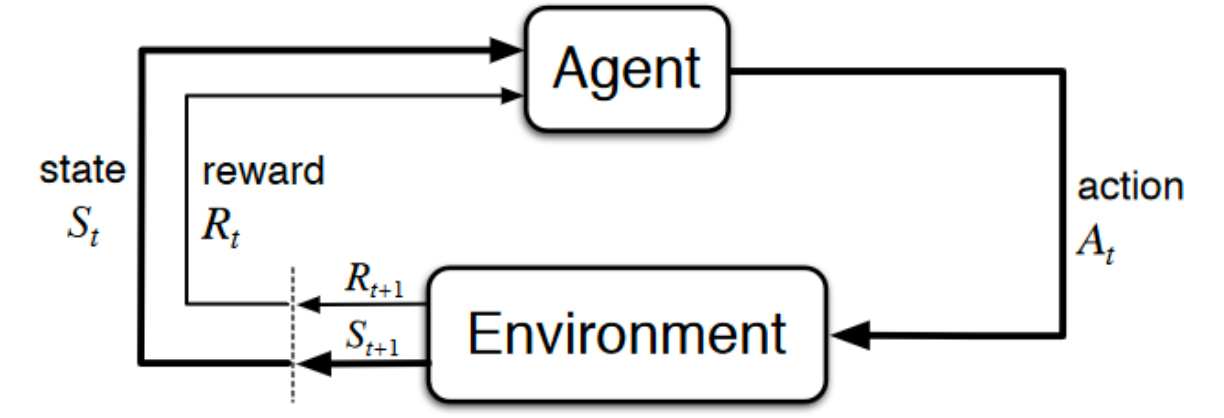
\includegraphics[width=0.7\textwidth]{model.png}
    \end{center}
      \caption{Teşvik Öğrenme Algoritması Modeli \cite{model}}
\end{figure}

\begin{enumerate}
    \item \textbf{Agent (Ajan):} Karar veren, öğrenen,  eylemleri belirleyen ve ödülü maksimize etmeye çalışan yapay zekadır.

    \item \textbf{Environment (Çevre):} Ajanın kararlarının etkileşimde bulunduğu ve ona geri bildirim sağlayan simülasyon ortamıdır.

    \item \textbf{State:} Zaman (t) anındaki çevrenin durumu ya da ajanın o andaki gözlemini temsil eder.

    \item \textbf{Action:} Ajanın zaman (t) anında yapmayı seçtiği eylemdir.

    \item \textbf{Reward:} Ajanın (t+1) anındaki eylemi sonucunda elde ettiği ödüldür

    \item \textbf{Next State:} Ajanın eylemi sonucunda çevrenin ulaştığı sonraki durumdur.
\end{enumerate}

\newpage

\section{Kurulum Aşamaları}
\rule{\textwidth}{0.5pt}
\begin{enumerate}
    \item cmd yani komut istemi çalıştırılır ve cd (dizini değiştir) komutuyla projenin olduğu dosya açılır.
    
    \item Dosyanın içinde venv adında bir virtual environment (sanal ortam) oluşturulur. Bu sayede python kullanılan başka bir proje ile karışıklık yaşanmasını önlenir.
    
    \item Oluşturulan sanal ortam aktive edilir.
    
    \item Python Package Installer (pip) güncel olup olmadığı kontrol edilir.
    
    \item ML-Agents paketi kurulur.

    \item Python torch kütüphanesi ve torch içindeki görüntü ve ses işleme kütüphanesi kurulur.
    
    \item protobuf 3.20.3 sürümü kurlur. Protobuf, veri transfer protokolü olup diğer protokollere göre daha hızlıdır.
    
    \item Packaging kütüphanesi kurulur. Bu kütüphane, python paketleri oluşturma, dağıtma ve sürümleme işlemlerini kolaylaştırır.
    
    \item Unity projesi açılıp Package Manager kısmından mlagents paketi aktif edilir.
    
    \item Boş bir nesne üretip bu nesnenin component kısmından ML-Agents aktif edilip edilmediği kontrol edilir.
    
\end{enumerate}

\newpage

\section{ML-Agents Bileşenleri}
\rule{\textwidth}{0.5pt}
\begin{enumerate}
    \item \textbf {Behavior Parameters:} Ajanların davranışlarını ve öğrenme süreçlerini kontrol etmek için kullanılan parametrelerin ayarlandığı bir bileşendir.
    \item \textbf {Buffer Sensor:} Çeşitli veri türlerini depolamak ve işlemek için kullanılan bir sensördür.
    \item \textbf {Camera Sensor:} Oyun dünyasını görsel veri olarak almak için kamera görüntülerini kullanan bir sensördür.
    \item \textbf {Decision Requester:} Ajanların kararlarını gerektiğinde talep etmelerini sağlayan bir bileşendir.
    \item \textbf {Demonstration Recorder:} Eğitim için insanların gerçekleştirdiği oyun hareketlerini kaydetmek ve kullanmak için bir kayıt cihazıdır.
    \item \textbf {Grid Sensor:} Grid tabanlı oyunlarda çevre bilgisini algılamak için kullanılan bir sensördür.
    \item \textbf {Match 3 Actuator:} Match 3 tarzı oyunlarda (Candy Crush) eylemleri gerçekleştirmek için kullanılan bir bileşendir.
    \item \textbf {Match 3 Sensor:} Match 3 tarzı oyunlarda oyun durumunu algılamak için kullanılan bir sensördür.
    \item \textbf {Ray Perception Sensor 2D/3D:} 2 boyutlu veya 3 boyutlu ortamlarda nesneleri algılamak için kullanılan bir sensördür.
    \item \textbf {Render Texture Sensor:} Görüntüleri işlemek için render texture'ları kullanarak veri sağlayan bir sensördür.
    \item \textbf {Vector Sensor:} Özel bir vektör verisiyle ajanlara çevre bilgisi sağlayan bir sensördür.\\[15pt]
\end{enumerate}

\begin{figure}
    \begin{center}
        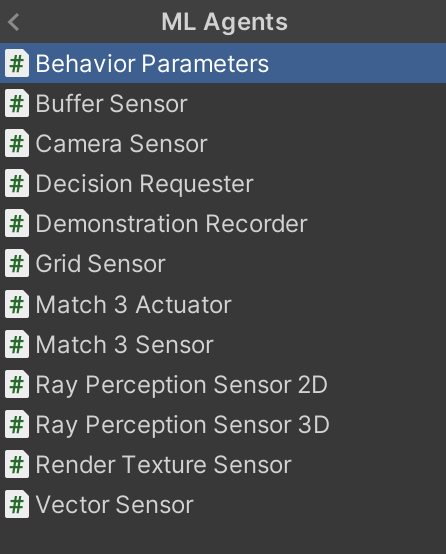
\includegraphics[width=0.9\textwidth]{mlagentcomponents.png}
    \end{center}
      \caption{ML-Agents Bileşenleri}
\end{figure}

\newpage

\section{ML-Agents Hareket Projesi}
\rule{\textwidth}{0.5pt}
Platform üzerinde mavi agentin hedeflediği mor renkli ödüller yer alır \cite{theashbot}. Bunların yanında görünmeyen ancak temas edildiğinde ceza uygulayan duvarlar da bulunmaktadır. Platformun rengi, Agent'ın etkileşimlerine göre değişmektedir. Ödül alındığında platform yeşile, duvara çarpıldığında kırmızıya dönüşür. Bu tasarım, agentin belirlenen hedeflere ulaşmasına teşvik ederken, aynı zamanda negatif etkileşimlerden kaçınma yeteneğini geliştirmeyi amaçlamaktadır. \\[5pt]

\begin{figure}[h]
    \begin{center}
        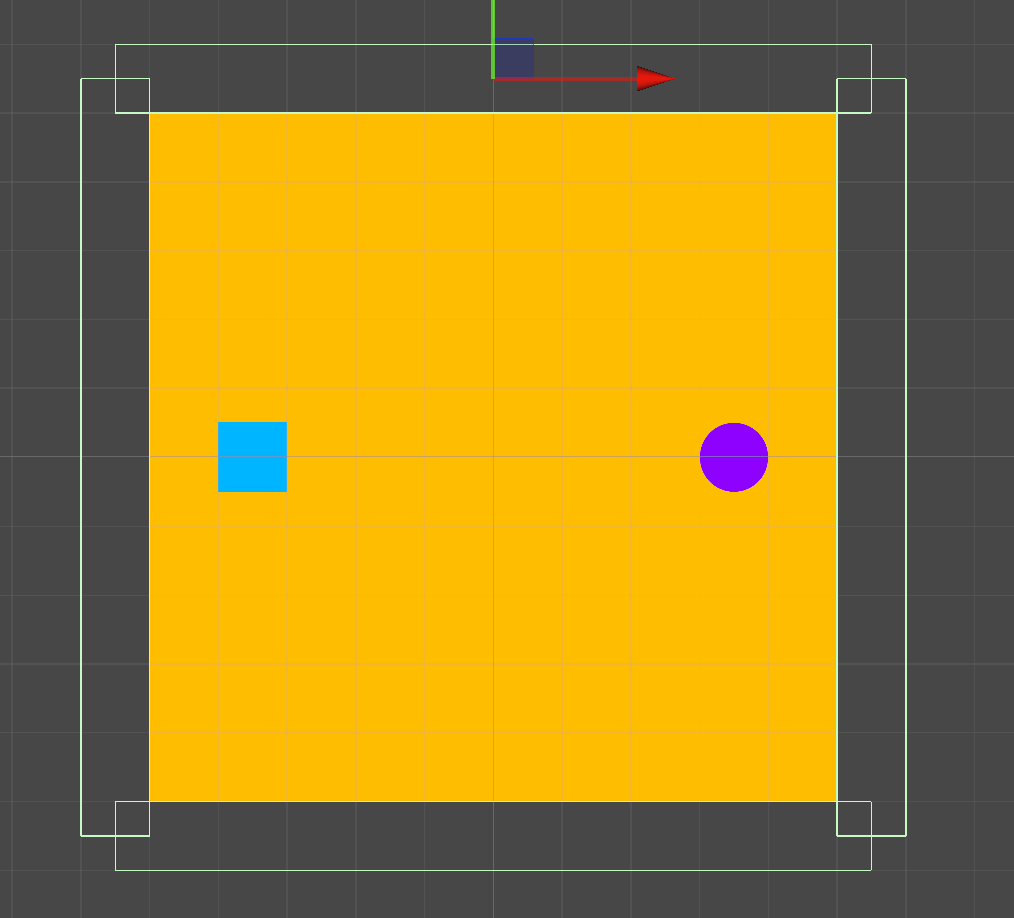
\includegraphics[width=0.8\textwidth]{duvar.png}
    \end{center}
      \caption{Hareket Projesi Bölüm Tasarımı}
\end{figure}

\newpage

\section{Proje Nesneleri}
\rule{\textwidth}{0.5pt}
Projenin bu kısmında kullanmak üzere dört adet nesne seçilmiştir. Seçilen nesneler platform, agent, ödül ve duvarlardır. Agent hareket ederek ödüle ulaşmayı hedefler fakat bu süreçte duvarlara temas ederse en baştan başlamak zorundadır.\\[5pt]

\begin{figure}[h]
    \begin{center}
        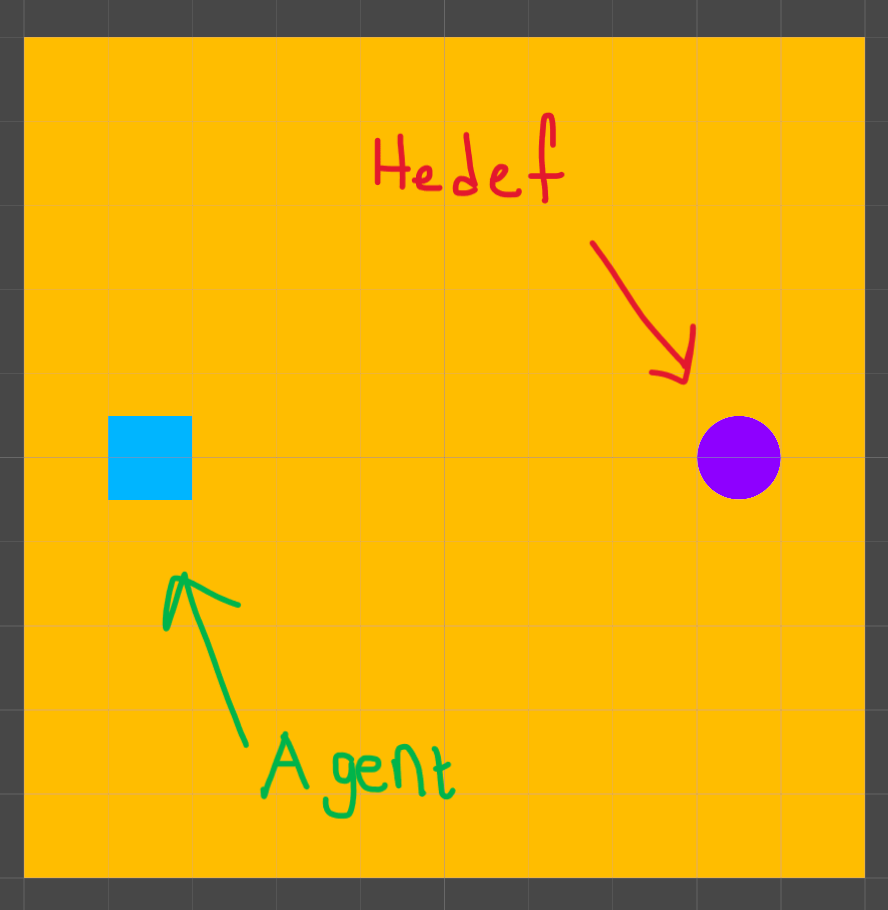
\includegraphics[width=0.9\textwidth]{agent_hedef.png}
    \end{center}
      \caption{Agent ve Hedef}
\end{figure}

\newpage

\section{ML-Agents Davranışları}
\rule{\textwidth}{0.5pt}
Agent hedefe ulaşmak için bir çok kez deneme yapmalıdır. Simulasyon hızlandırılmış olsada daha da hzılandırmak için oluşturulan bölüm koyalanarak toplamda aynı bölümden dokuz tane oluşturulmuştur. Böylece dokuz ajan aynı anda eğitilir. \\[5pt]

\begin{figure}[h]
    \begin{center}
        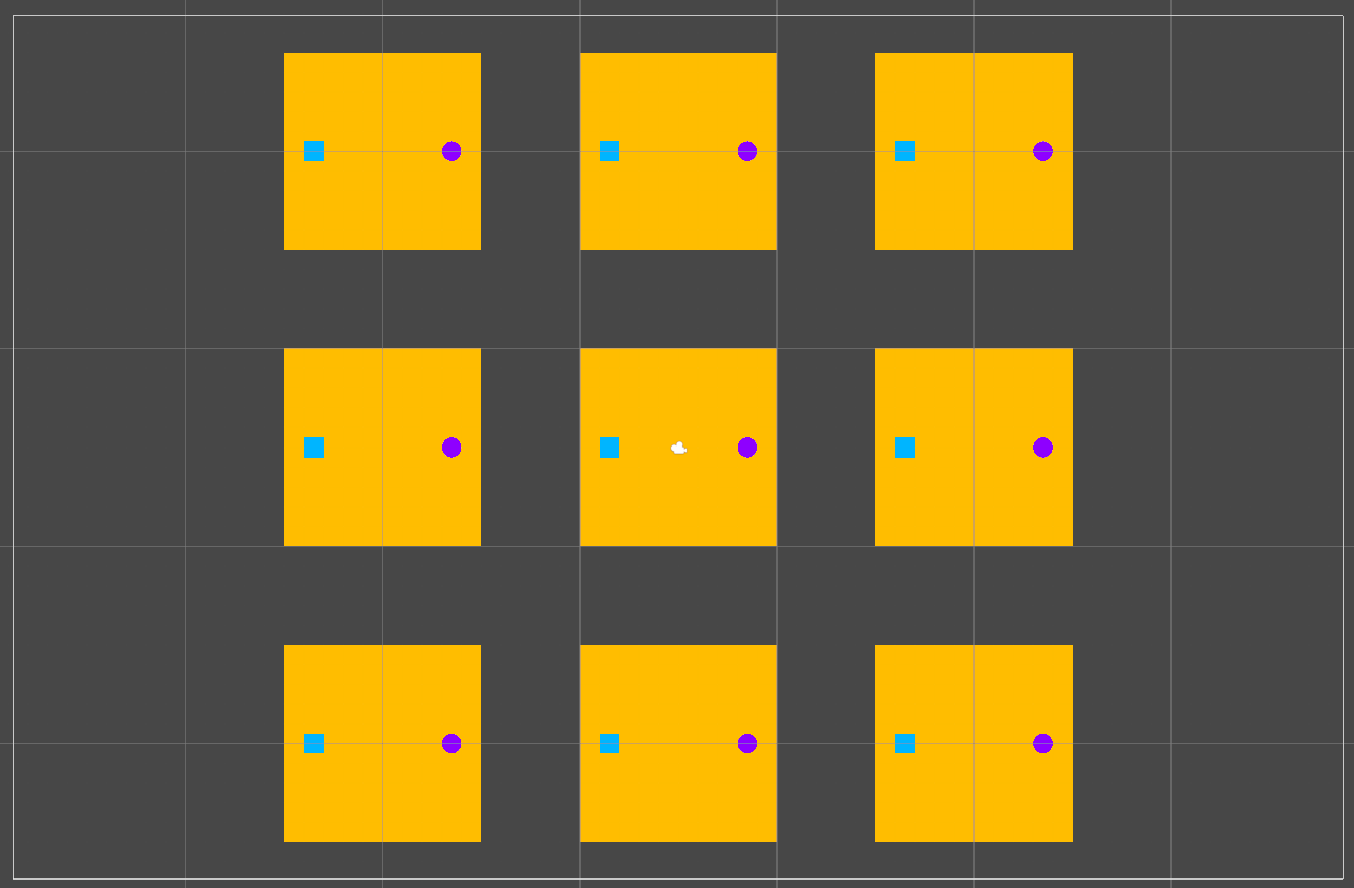
\includegraphics[width=1.1\textwidth]{coklu_bolum.png}
    \end{center}
      \caption{Çoklu Bölüm}
\end{figure}

\newpage

\section{Araç Kontrolleri Öğrenme Projesi}
\rule{\textwidth}{0.5pt}
\par Hareket Projesine benzer olarak, platform üzerinde agentin hedeflediği mor renkli ödüller yer alır. Bu ödüllerin yeri her denemede rastgele olacak şekilde değişir. Araç duvara çarparsa ceza puanı alır ve yeniden başlar, araç hedefe ulaşırsa ödül puanı alır ve yeniden başlar. Platformun rengi, Agent'ın etkileşimlerine göre değişmektedir. Ödül alındığında platform yeşile, duvara temas edildiğinde kırmızıya dönüşür. Bu tasarım, ajanların basit araç kontrollerini öğrenmesini sağlar.
\newline
\par flyyufelix adlı github kullanıcısının yaptığı "donkeyrl" projesinde\cite{flyyufelix} Donkey Car adı verilen bir arabanın bir pist etrafında RL kullanarak kendi kendine dönmesini sağlamıştır. Bu projede Double Deep Q Learning (DDQN) kullanılmıştır. DDQN, bir ajanın çevresiyle etkileşime girerek belirli bir durumda alabileceği eylemler arasında en uygun olanını seçmeyi öğrenen bir güçlendirme öğrenme algoritmasıdır.\\[15pt]

\begin{figure}[h]
    \begin{center}
        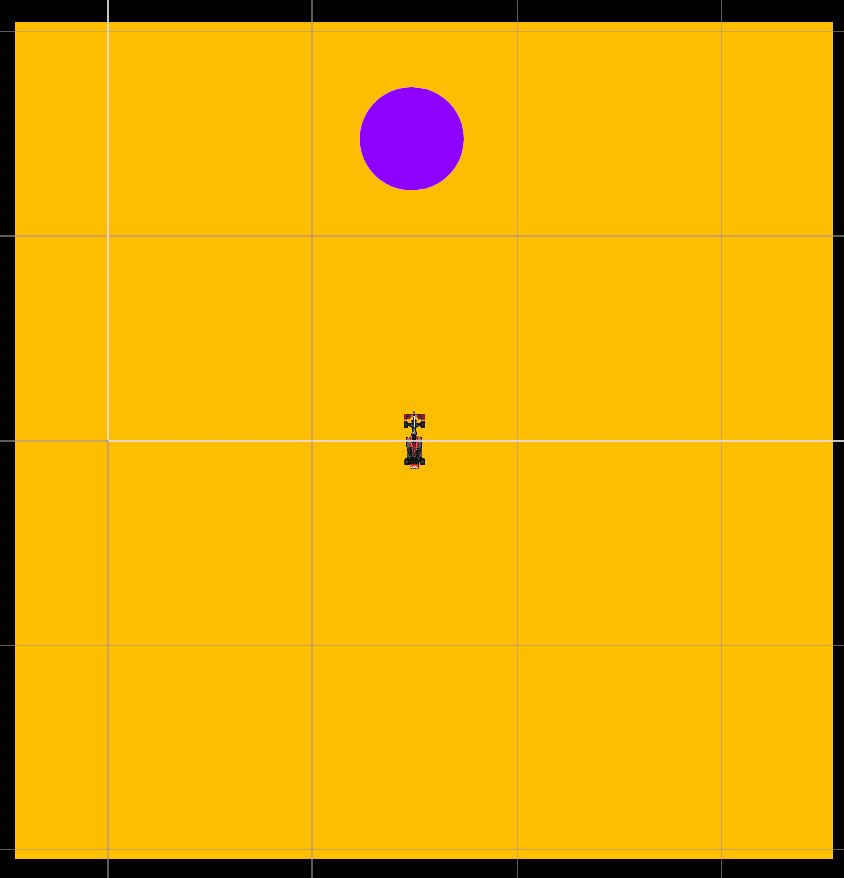
\includegraphics[width=0.7\textwidth]{tek-map.png}
    \end{center}
      \caption{Araç Kontrolleri Öğrenme Projesi Bölüm Tasarımı}
\end{figure}

\newpage

\section{Araç ve Ajan Kontrolleri}
\rule{\textwidth}{0.5pt}
\par Önceden carInput isminde başka bir koddan alınan girdiler, ajan kodunun içindeki X ekseni ve Y ekseni olarak ajan hareketlerinden alındı. Böylece ajanların araba kontrollerine erişimi sağlandı. 
\newline
\par Ajanın kullancı tarafından kontrol edilip edilemediğini, ajanın kaç eksende hareket yaptığını, eğitilen beynin ajana aktarıldığı ve diğer bir çok ayarların yapıldığı kısım Behavior Parameters olarak adlandırılır. Bu özellik ML-Agents ile birlikte gelir.\\[5pt]


\begin{figure}[h]
    \begin{center}
        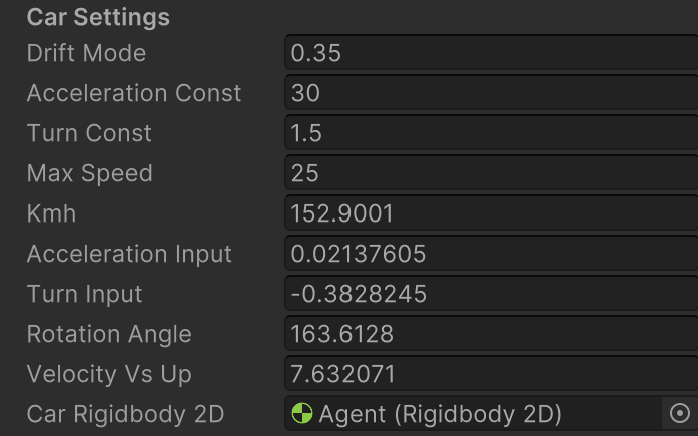
\includegraphics[width=0.65\textwidth]{kontrol.png}
    \end{center}
      \caption{Araba Kontrolleri}
\end{figure}

\begin{figure}[h]
  \centering
  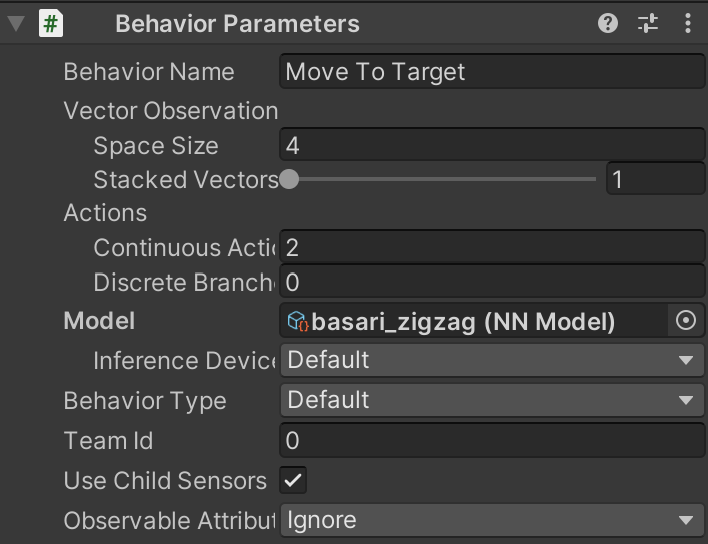
\includegraphics[width=0.65\textwidth]{behavior.png}
  \caption{Behavior Parameters}
\end{figure}

\par\textbf{Behavior Type:} Agent'ın kullancı tarafından kontrol edilip edilemediğini değiştiren bir özelliktir. Agent'ı kullanıcının  yönetmesi isteniyorsa heuristic only seçeneği seçilmelidir. Agent'a dışarıdan herhangi bir müdehalede bulunmadan hedefe ulaşması isteniliyorsa inference only seçeneği seçilmelidir.
    \newline

\begin{figure}[h]
  \centering
  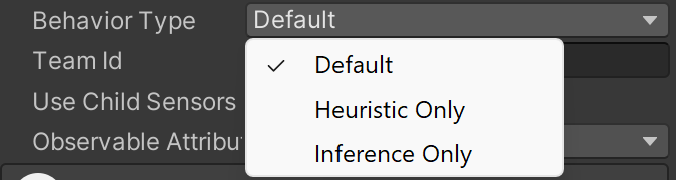
\includegraphics[width=0.9\textwidth]{behavior_type.png}
  \caption{Behavior Type}
\end{figure}

\vspace{1cm}

\par\textbf{Space Size:} Agent'ın sahip olduğu davranışları belirleyen ve yönlendiren bir özelliktir. Bazı durumlarda Agent'ın farklı davranışlar sergilemesi istenebilir. Bu durumda, her bir nesner için farklı davranışlar tanımlanması gerekir. Bu projede Agent ve Ödül olarak iki hareketli nesne olduğundan her iki nesnenin de x ve y eksenindeki hareketleri almak için Space Size özelliği dört olarak ayarlanır.
    \newline

\begin{figure}[h]
  \centering
  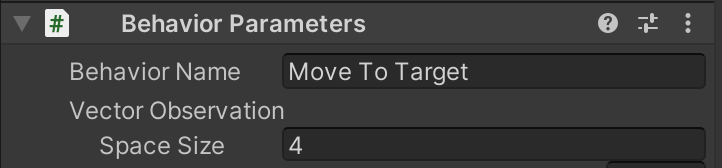
\includegraphics[width=0.9\textwidth]{space_size.png}
  \caption{Space Size}
\end{figure}

\vspace{1cm}

\newpage

\section{Beyin Oluşturma Kaydetme ve Yükleme}
\rule{\textwidth}{0.5pt}
\begin{enumerate}
\item  Unity projesi çalıştırıldığından itibaren Agentlar öğrenmeye başlar. Öğrenmiş olan bu beyin, proje dosyasının içindedir\\[5pt]

\begin{figure}[h]
  \centering
  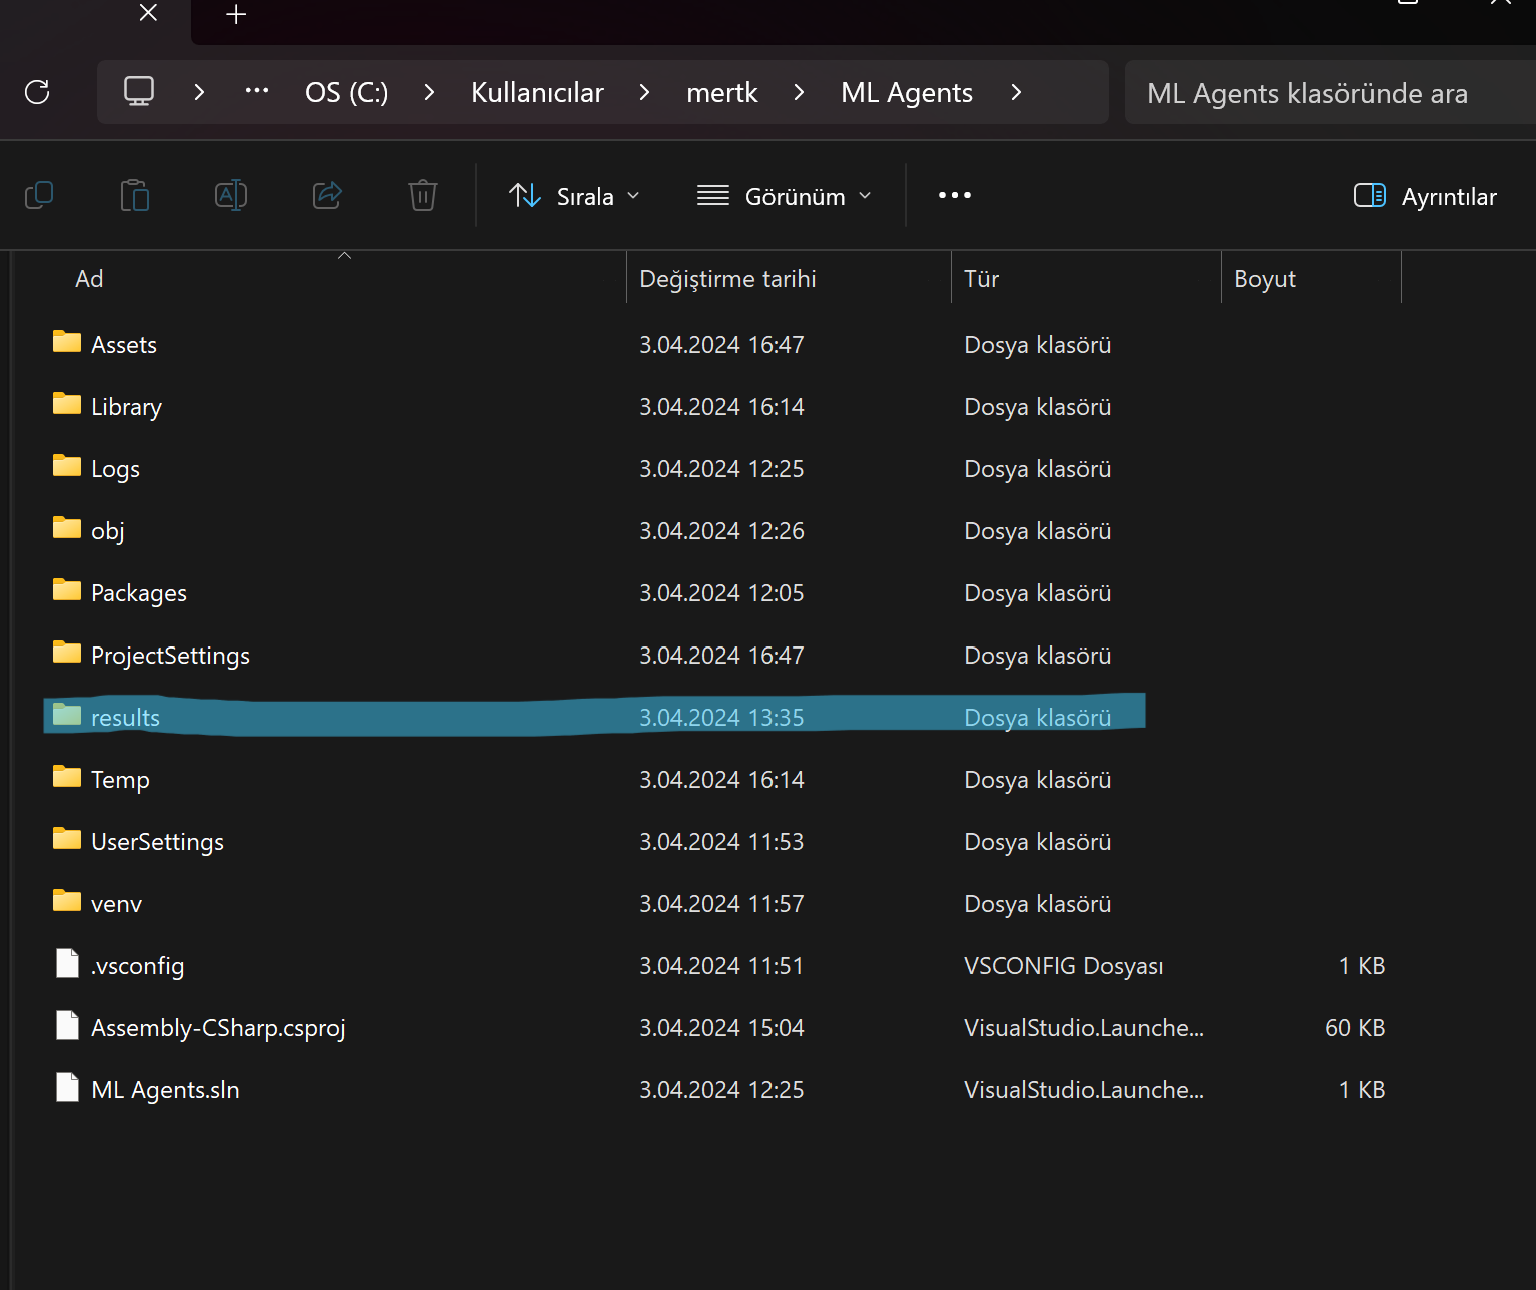
\includegraphics[width=1\textwidth]{results.png}
  \caption{Proje Dosyaları}
\end{figure}

\vspace{1cm}

\begin{figure}[h]
  \centering
  
\includegraphics[width=1\textwidth]{beyin.png}
  \caption{Beyin Dosyası}
\end{figure}

\newpage

\item Result dosyasının içindeki beyin, proje dosyasının içindeki Assets klasörüne kopyalanır. Kopyalanan bu beyin Unity içerisinde Assets kısmında görülebilir.

\begin{figure}[h]
  \centering
  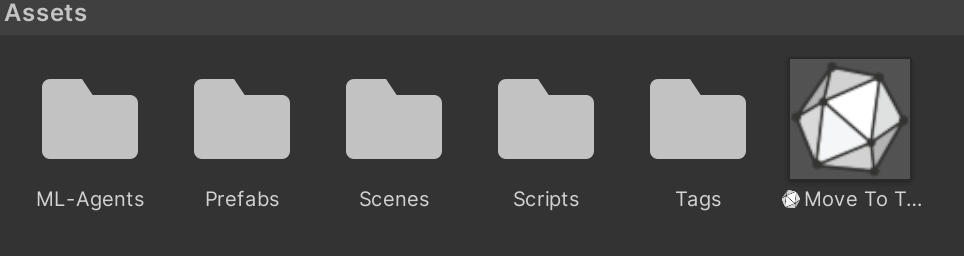
\includegraphics[width=1\textwidth]{assets_beyin.png}
  \caption{Assets Klasörü}
\end{figure}

\vspace{1cm}

\item Agent altında, Behavior Parameters bileşeninin içindeki, Model adındaki değişkene Assets klasöründeki beyin atanır. Böylece önceden eğitilen bir Agent'ı projeye eklemiş oluruz.

\begin{figure}[h]
  \centering
  
\includegraphics[width=1\textwidth]{brain_model.png}
  \caption{Model Değişkeni}
\end{figure}

\end{enumerate}

\newpage

\section{Başarılı ve Başarısız Oranı}
\rule{\textwidth}{0.5pt}

\par  Ekranın sol üst kısmında başarılı deneme sayısını, başarısız deneme sayısını, başarılı ve başarısız deneme sayısı arasındaki farkı ve başarı oranını gösteren bir panel yer almaktadır. Bu panel sayesinde deneme sayısı arttıkça başarı oranının arttığı gözlemlenebilir.\\[5pt]

\begin{figure}[h]
  \centering
  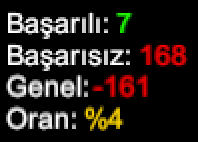
\includegraphics[width=0.7\textwidth]{basarisiz.png}
  \caption{Az Deneme Sayısı}
\end{figure}

\begin{figure}[h]
  \centering
  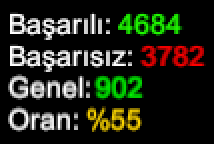
\includegraphics[width=0.7\textwidth]{basarili.png}
  \caption{Çok Deneme Sayısı}
\end{figure}

\newpage

\par Eğitim tamamlandıktan sonra TensorBoard yardımıyla sonuçlar grafik halinde görüntülenebilir. Aşağıdaki grafikler eğitilmiş bir beyine aittir.\\[5pt]

\begin{figure}[h]
  \centering
  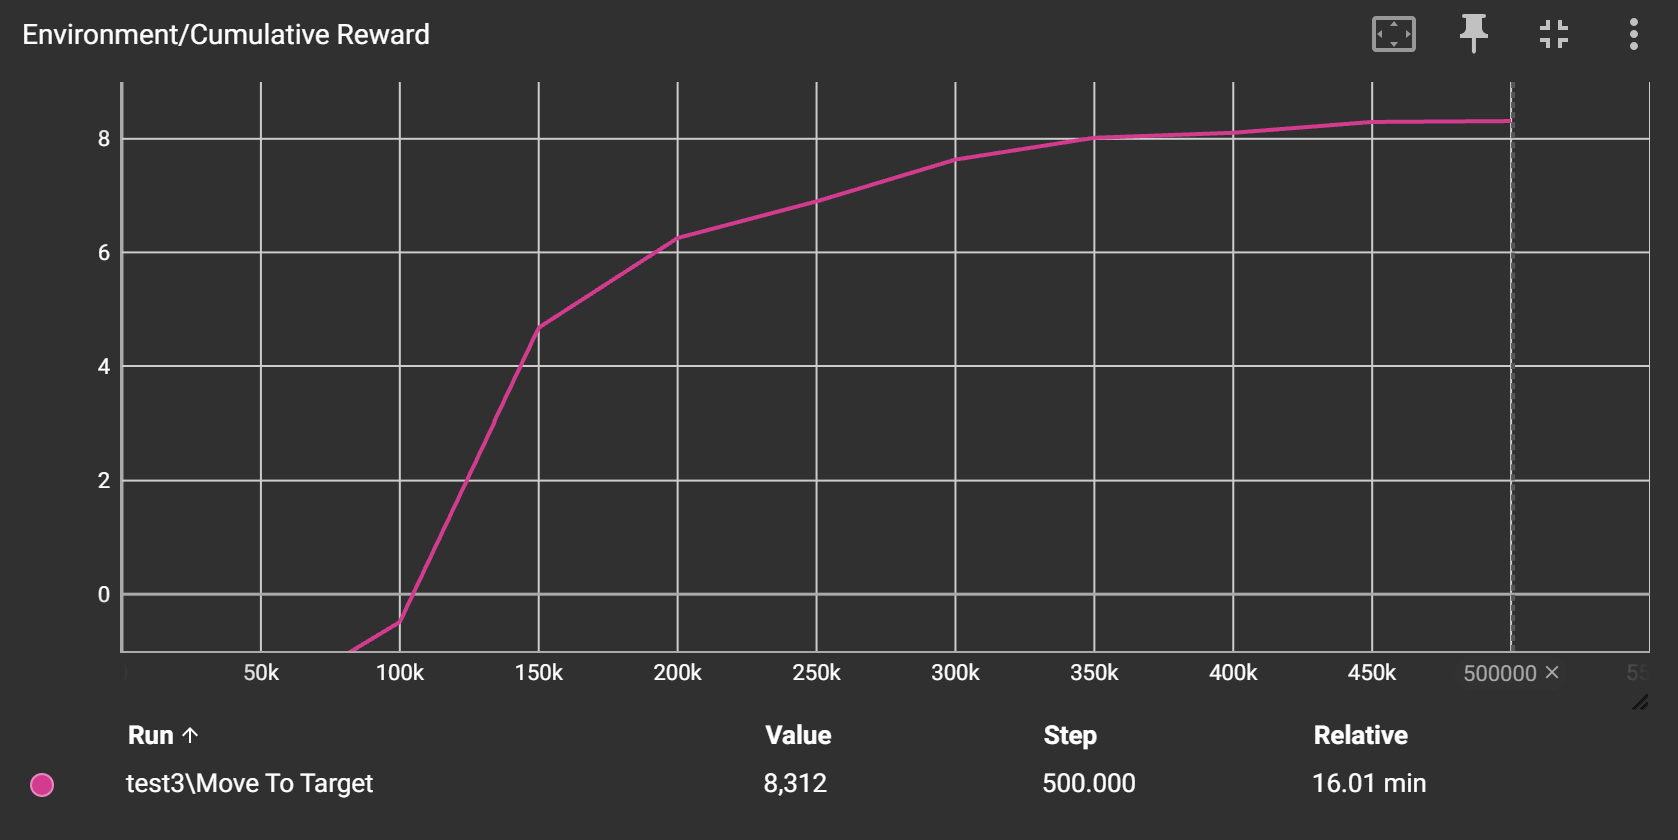
\includegraphics[width=0.9\textwidth]{reward-grap.png}
  \caption{Toplam Ödül Sayısı Grafiği}
\end{figure}

\begin{figure}[h]
  \centering
  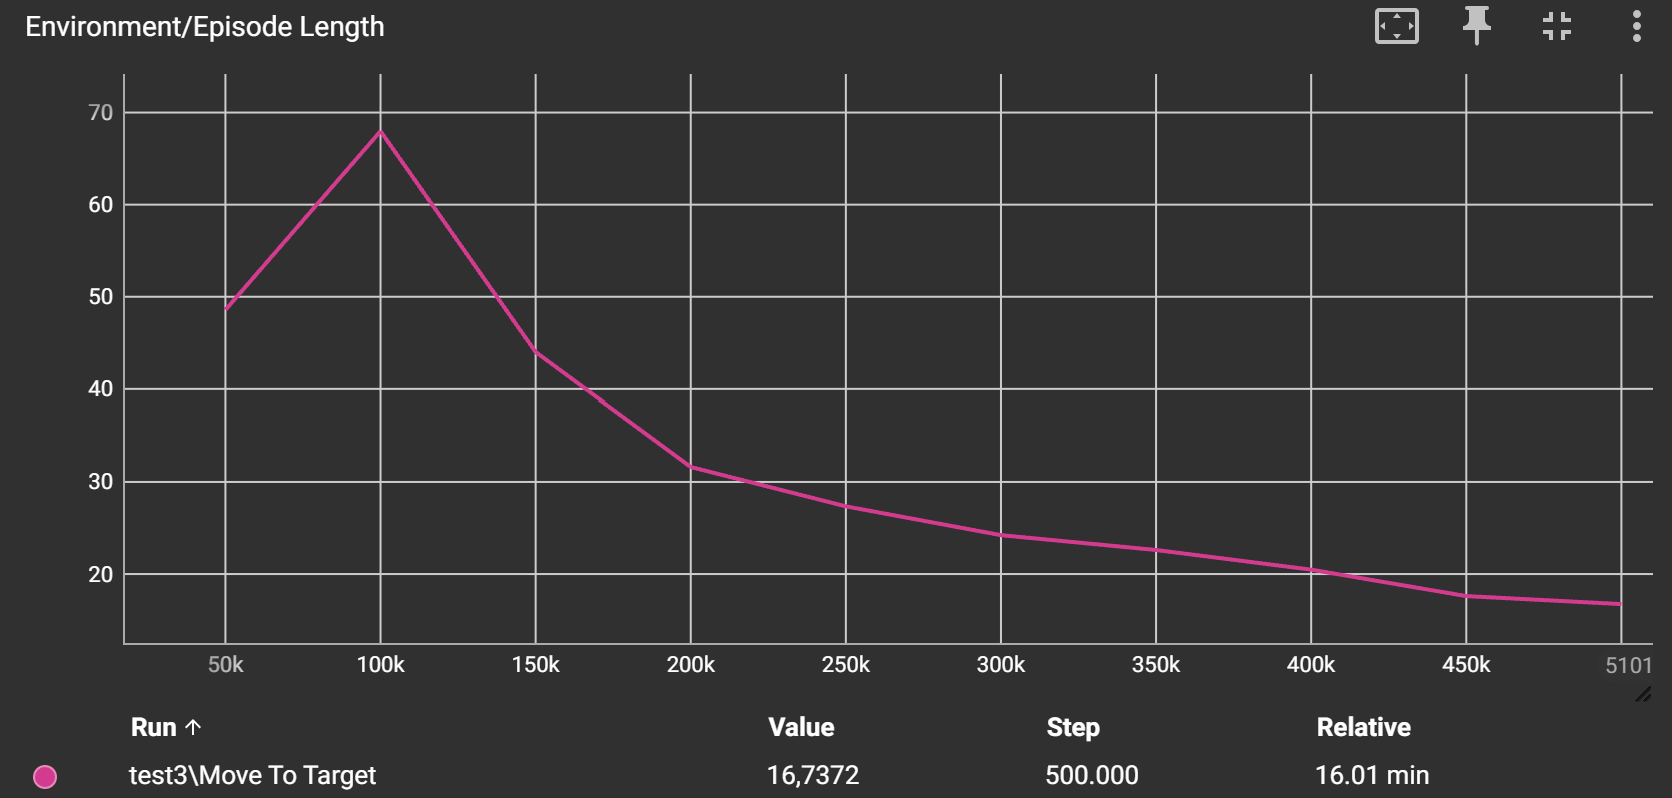
\includegraphics[width=0.9\textwidth]{episode-len.png}
  \caption{Bölüm Uzunluğu Grafiği}
\end{figure}

\newpage

\section{Sonuç}
\rule{\textwidth}{0.5pt}
\par Bu çalışma, Unity'nin ML-Agents kütüphanesi kullanılarak Python ve PyTorch ile geliştirilen bir yapay zeka projesine odaklanmaktadır. Projenin amacı, araç sürmeyi öğrenen ve geliştiren bir yapay zeka modeli oluşturmaktır. Çalışmanın sonuçları, ajanların çevreleriyle etkileşime girerek araba kontrolü öğrenmesini sağladığını göstermektedir. Eğitim sonucunda elde edilen başarı oranları ve ödül grafiği incelendiğinde, ajanların belirlenen hedeflere ulaşma yeteneklerinin arttığı ve bölüm tamamlama süresinin azaldığı görülmektedir. Bu sonuçlar, ML-Agents kütüphanesi kullanarak yapay zeka modellerinin eğitilmesinin ve çeşitli görevlerin başarılı bir şekilde öğrenilmesinin mümkün olduğunu göstermektedir. 

\newpage

\bibliographystyle{ieeetr}
\bibliography{ref}

\end{document}
